%
% Draft  document ppcell.tex
% Looks at how dynamics of pre-papilla cell numbers affects follicle development
%
 
\documentclass[titlepage]{article}  % Latex2e
\usepackage{graphicx,lscape,subfigure}
\usepackage{tikz}
\usepackage{bm,longtable}
\usepackage{textcomp}
 

\title{Dynamics of pre-papilla cell numbers in sheep foetus and effect on follicle development}
\author{Neville Jackson and Philip Moore}
\date{7 Mar 2018} 

 
\begin{document} 


 
\maketitle      
\tableofcontents

$\newcommand{\E}{\mathrm{E}}$
$\newcommand{\Var}{\mathrm{Var}}$
$\newcommand{\Cov}{\mathrm{Cov}}$ 
$\newcommand{\SD}{\mathrm{SD}}$ 

\clearpage
\section{Introduction} 
It has been shown that there  exists in the dermis of the the developing sheep foetus a population of cells, known as pre-papilla cells, which migrate to the site s of follicle formation and differentiate, ending up in the papilla of the follicle bulb ( Moore, etal (1989)~\cite{moor:89}, Moore etal (1998)~\cite{moor:98}). These cells are of mesenchymal origin, in contrast to all other tissue in the follicle, which arises from the epidermis. It is thought that these cells control follicle development, and, in particular, that the number of papilla cells which end up in a follicle bulb  at least partly determines follicle size and fibre diameter, and perhaps other follicle and fibre characteristics.

There also exist in the foetal dermis, specific locations, known as 'sites' , at which follicles can develop by attracting a number of pre-papilla cells, and intitating epidermal downgrowth. Not all follicles form at 'sites'. Primary follicles (P), and secondary-original (So) follicles (Fraser and Short(1960)~\cite{fras:60}) form at 'sites', secondary-derived follicles (Sd) form as outgrowths from the wall of So follicles, and produce fibres which emerge from a common follicle opening at the skin surface. Primary follicle initiation starts first ( at about 64 days), secondary original follicles start to form at around 85 days, and, when all sites are used up, Sd follicles form from about 100 days, and almost all follicle initiation is complete before birth at around 150 days. 

While follicles are initiating the population of pre-papilla cells in the dermis is undergoing dynamic change. Cells are moving out of the population, to migrate to the sites of follicles, and to differentiate. Cells are also being added to the population by mitosis.

\section{Materials and Methods}

\subsection{Measurements}


\subsection{Statistical Methods}
Data were imported into the R statistical program~\cite{rprog:13} .

\subsection{Growth curve simulation}
\label{sec:growth}
We need to model the growth of a lamb from a day 60 foetus to adulthood. 
For this we use a generalised logistic function. This is an 'S' or sigmoid shaped curve. It is also known ar Richard's curve. It was originally developed for growth modelling. The equation is
\begin{equation}
\label{eqn:logi}
Y_{t} = A + \frac{K - A}{(C + Q \exp{-B t})^(1/\nu)}
\end{equation}
where 
\begin{description}
\item[$Y_{t}$] is body weight at time $t$ in gm
\item[$A$] is the lower asymptote of the curve - ie zero if curve starts at day zero
\item[$K$] is the upper asymptote of the curve - ie adult weight if the curve goes to mature age
\item[$B$] is the growth rate 
\item[$\nu$] $>0$ positions the maximum growth rate in relation to age
\item[$Q$] is the Y value at the point of inflection - ie at the greatest growth rate
\item[$C$] is typically set to 1
\end{description}

What we need to do is to find an appropriate set of parameters for this equation. We start with some foetal weight data from Metcalf etal(1962)~\cite{metc:62}. These data are for Merino sheep.  Figure~\ref{fig:mfbwagefit} shows these data with a set of points generated by equation~\ref{eqn:logi} superimposed. 
%\documentclass{article}
%\usepackage{graphicx,subfigure}
%\begin{document}

\begin{figure}[!h]
  \centering
   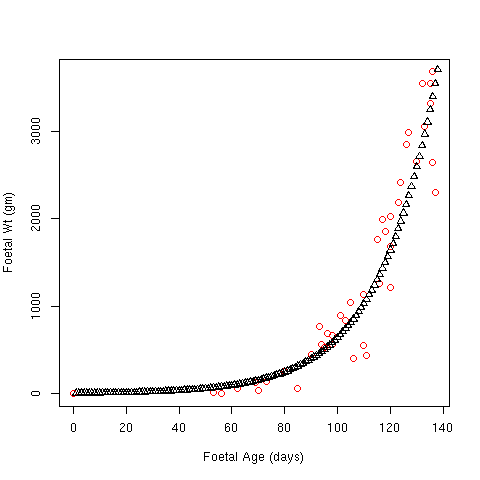
\includegraphics[width=0.9\textwidth]{mfbwagefit.png}
%  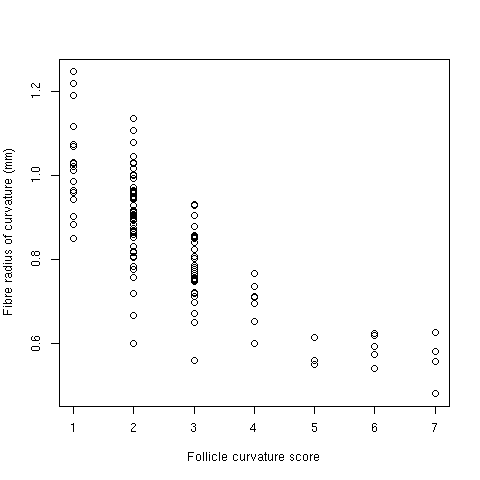
\includegraphics{ofdamm.png}
  \caption{Plot of foetal body weight data from Metcalf etal(1962)~\cite{metc:62} (red circles) with the simulated foetal bodyweights from our generalised logistic equation~\ref{eqn:logi} superimposed (black triangles). Parameters for the logistic equation were, $A=0$, $K=45000$, $B=.048$, $\nu=1$, $Q=8000$,$C=1$. Points were calculated over the range zero to 150 days}
  \label{fig:mfbwagefit}
\end{figure}

%\end{document}


The agreement is satisfactory. We therefore accept these parameters as a first approximation for the prenatal part of the curve.

We now need to look at postnatal growth, that is the latter part of the sigmoid growth curve. We have some data on Merino lambs from birth up to 20 weeks ( 140 days) from Taplin and Everitt(1962)~\cite{tapl:62}. These  data have 4 groups of lambs with different feeding regimes. We plot all the data on top of Figure~\ref{fig:mfbwagefit} in Figure~\ref{fig:mlbwagefit}
%\documentclass{article}
%\usepackage{graphicx,subfigure}
%\begin{document}

\begin{figure}[!h]
  \centering
   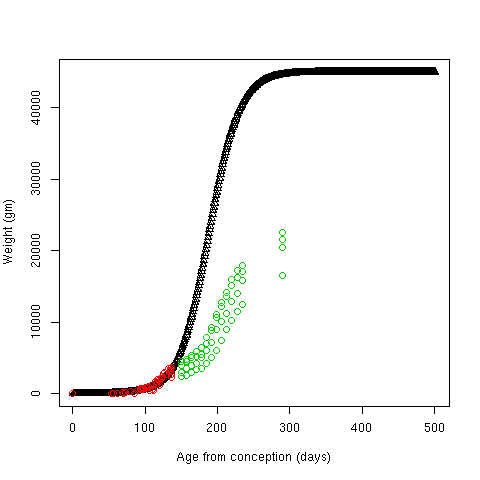
\includegraphics[width=0.9\textwidth]{lwagefit2.png}
%  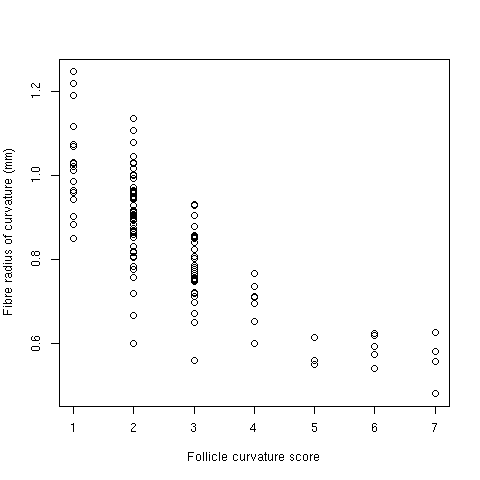
\includegraphics{ofdamm.png}
  \caption{Plot of foetal body weight data from Metcalf etal(1962)~\cite{metc:62} (red circles) with the simulated foetal bodyweights from our generalised logistic equation~\ref{eqn:logi} superimposed (black triangles). Postnatal growth data from Taplin and Everitt(1962)~\cite{tapl:62} are superimposed as green circles.  Parameters for the logistic equation were, $A=0$, $K=45000$, $B=.048$, $\nu=1$, $Q=8000$,$C=1$. Points were calculated over the range zero to 500 days}
  \label{fig:mlbwagefit}
\end{figure}

%\end{document}


We see that the theoretical growth curve does not match the postnatal data because it is too steep. So we modify the parameters as follows. We change the growth rate parameter (B) to 0.028, and the parameter which positions the point of inflection (Q) to 1000. This leads to the plot shown in Figure~\ref{fig:mlbwagefit3}
%\documentclass{article}
%\usepackage{graphicx,subfigure}
%\begin{document}

\begin{figure}[!h]
  \centering
   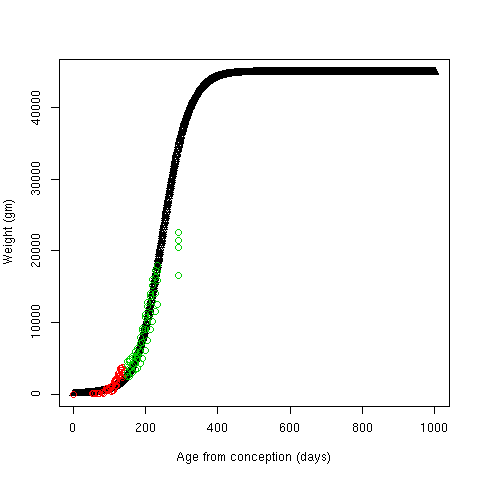
\includegraphics[width=0.9\textwidth]{lwagefit3.png}
%  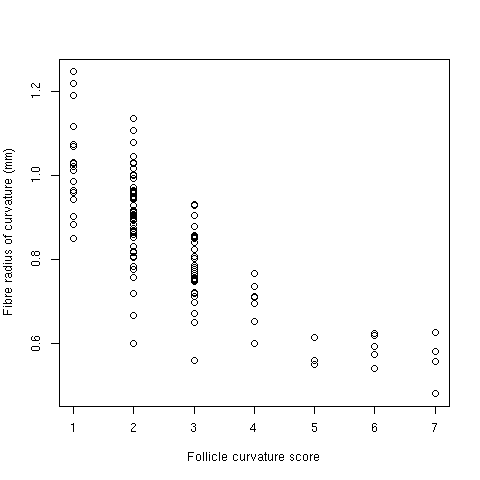
\includegraphics{ofdamm.png}
  \caption{Plot of foetal body weight data from Metcalf etal(1962)~\cite{metc:62} (red circles) with the simulated foetal bodyweights from our generalised logistic equation~\ref{eqn:logi} superimposed (black triangles). Postnatal growth data from Taplin and Everitt(1962)~\cite{tapl:62} are superimposed as green circles.  Parameters for the logistic equation were, $A=0$, $K=45000$, $B=.028$, $\nu=1$, $Q=1000$,$C=1$. Points were calculated over the range zero to 500 days}
  \label{fig:mlbwagefit3}
\end{figure}

%\end{document}


We see that our theoretical growth curve now follows the points well, except for the 20 week ( post weaning) weights shown as green dots to the right of the curve. Sheep grow at a slower rate as they mature. It is not possible with a sigmoidal curve like the Richards curve to make the growth rate slower above the point of inflection than below it. The curve is symmetric, in that sense. From the point of view of our model this is not a significant issue, the important thing being to get the prenatal and neonatal growth pattern realistic. We have done that, so we are going to stop here and use the growth curve of Figure ~\ref{fig:mlbwagefit3}.  This is an "average" curve. We can study small perterbations from the average ( eg a faster growth rate) simply by varying its parameters.

\section{Calculating the dynamics of pre-papilla cell numbers}
\label{sec:calc}
 Before follicles start to initiate there is a population of pre-papilla cells. This populaton is characterised by its population size ( cell number) $C_{n}$
and its mitotic rate which we describe as its cell birth probability (probability that a cell chosen at random divides in a unit time ) $C_{b}$.

 The first follicles to form are called primary follicles. This activity begins at locations called 'sites'. There are a definite number ($L_{p}$) of primary follicle sites on a sheep's skin. Primary follicle initiation begins at a foetal age of around 64 days ($T_{p}$), and ends when all the primary follicle 'sites' are used.

Each primary follicle formed uses a number of pre-papilla cells. We call the average number of pre-papilla cells per primary follicle $C_{p}$. The rate at which follicles form we designate $F_{r}$. It is not dependent on time, or on the type of follicle being formed, or on the number of available sites or pre-papilla cells. It is simply the differentiation rate of follicles ( no of follicles per unit skin area per day). 

We start calculating at a given day ($t$) , and while primary follicles are initiating ( ie beginning at time $T_{p}$, the time at which primary inittiation starts) we calculate
\begin{eqnarray}
\label{eqn:prim}
P_{t} & = & P_{t-1} +  F_{r} * S_{t} \\
\label{eqn:prim2}
D_{t} & = & P_{t} * C_{p} \\
\label{eqn:prim3}
(C_{n})_{t+1} & = & (C_{n})_{t} + C_{b} * (C_{n})_{t} + D_{t}
\end{eqnarray}
where 
\begin{description}
\item[$P_{t}$] is number of primary follicles formed in time interval $t$
\item[$D_{t}$] is number of pre-papilla cells which differentiate ( ie become papilla cells) in time interval $t$
\item[$S_{t}$] is the surface area of skin on the sheep at time t
\end{description}
This is a recurrence equation, because each time round depends on values in the previous time round. The equations can be evaluated sequentially, starting from time zero. The calculation in equations~\ref{eqn:prim}, ~\ref{eqn:prim2}, and ~\ref{eqn:prim3} continues until all of the primary follicle sites are utilized ( ie until $ P_{t} = L_{p} $). 

In the period between primary follicle intitation and secondary follicle initiation, there are no follicles formed, so no pre-papilla cells differentiate, but the pre-papilla cell population continues to multiply. So we have just one equation
\begin{equation}
\label{eqn:mult}
(C_{n})_{t+1}  =  (C_{n})_{t} + C_{b} * (C_{n})_{t}
\end{equation}
The calculation in equation~\ref{eqn:mult} continues until the time $t$ reaches  $T_{So}$.

When secondary original follicles begin to initiate ( ie beginning at time $t_{So}$ ) we calculate
\begin{eqnarray}
\label{eqn:so}
So_{t} & = & So_{t-1} +  F_{r} * S_{t} \\
\label{eqn:so2}
D_{t} & = & So_{t} * C_{s_{o}} \\
\label{eqn:so3}
(C_{n})_{t+1} & = & (C_{n})_{t} + C_{b} * (C_{n})_{t} + D_{t}
\end{eqnarray}
where
\begin{description}
\item[$So_{t}$] is number of primary follicles formed in time interval $t$
\item[$C_{s_{o}}$] is the average number of pre-papilla cells per So follicle.
\end{description}

The calculation in equations ~\ref{eqn:so}, ~\ref{eqn:so2}, and ~\ref{eqn:so3} continues until all of the So follicle sites are utilised. There are typically 3 So sites per P follicle site ( because the follicles form in trio groups (Carter(1943)~\cite{cart:43}). So So follicles continue to form until $ So_{t} = L_{So} $  where $L_{So} = 3 * L_{p} $. It would be unusual for the number of prepapilla cells $(C_{n})_{t}$ to exhaust before all So sites are utilised, in a Merino sheep, but this happens in non-Merino breeds. 

After all of the So sites are utilized, any remaining pre-papilla cells have nowhere specific on the epidermis to initiate a follicle downgrowth, so what happens is that they form follicles by branching from the stem of existing follicles. The branches are termed secondary derived (Sd) follicles after Hardy and Lyne(1956)~\cite{hard:56}

The initiation of Sd follicles continues immediately after all So sites are utilized, and continues until all of the remaining pre-papilla cells are differentiated. It is assumed that the initiation rate of Sd follicles is the same as that for follicles at sites. We calculate
\begin{eqnarray}
\label{eqn:sd}
Sd_{t} & = & Sd_{t-1} +  F_{r} * S_{t} \\
\label{eqn:sd2}
D_{t} & = & Sd_{t} * C_{s_{d}} \\
\label{eqn:sd3}
(C_{n})_{t+1} & = & (C_{n})_{t} + C_{b} * (C_{n})_{t} + D_{t}
\end{eqnarray}
where
\begin{description}
\item[$Sd_{t}$] is number of primary follicles formed in time interval $t$
\item[$C_{s_{d}}$] is the average number of pre-papilla cells per Sd follicle.
\end{description}
 
The calculation in equations ~\ref{eqn:sd}, ~\ref{eqn:sd2}, and ~\ref{eqn:sd3} continues until $(C_{n})_{t}$ reduces to zero.

When all pre-papilla cells are differentiated follicle development ceases. The numbers of follicles on the animal stay constant thereafter, but the density of follicles ( follicles per $mm^{2}$ of skin) varies because the animal continues to grow.  Adult densities are much lower than those observed in a lamb.

Equations~\ref{eqn:prim} to ~\ref{eqn:sd3} are a relatively simple sequence of calculations which are readily programmed. We have set up a calculation package using the R statistical software (R core Team (2013)~\cite{rprog:13}). It is available as the R package {\em ppcell}~\cite{jack:18} 




\section{Results}
We use the R package {\em ppcell} to calculate developmental outcomes in terms of follicle density and fibre diameter, given various asssumptions regarding the somwewhat large number of input parameters.

\subsection{The base set of assumed values for input parameters}
The full set of 20 starting parameters is shown in Table~\ref{tab:base}.
%\documentclass{article}
%\usepackage{lscape}
%\begin{document}

\begin{table}[htp]
\centering
\caption{Base input parameters for package {\em ppcell}, their definition, and assumed average values for a Merino sheep} 
\label{tab:base}
\vspace{0.1in}
\begin{tabular}{|p{0.5in}|p{2.0in}|p{1.2in}|p{0.5in}|}  \hline
     Parameter & Description  & Units & Average value  \\ 
\hline 
  A    & Lower growth asymptote  & $gm$ & 0 \\
  K    & Upper growth asymptote ( mature weight)  & $gm$ & 45000 \\
  B    & Growth rate             & log(gm) per day & 0.028 \\ 
 $\nu$ & Controls age at maximum growth rate & no units  & 1\\
  Q    & Controls weight at maximum growth rate & no units  & 1000\\
  C    & Controls upper asymptote & no units  & 1\\
\hline
  $S_{k}$ & Surface area constant for sheep & no units  & 9.0 \\
  $t_{0}$ & Zero time for calculations & days & 60  \\
  $t_{max}$ & Maximum time for calculations & days & 900 \\
  $\delta t$ & Time increment for calculations & days & 1  \\
  $L_{p}$  &  Number of primary follicle sites & number & 2e+06 \\
  $S_{o}/P$ & Number of So sites per P site & no units  & 3 \\
  $F_{r}$ & Follicle initiation rate per unit area per unit time & no per $cm^{2}$ per day  & 450\\
  $T_{P}$ & Start time for P follicle inititation & days & 64 \\
  $T_{So}$ & Start time for So follicle intiation & days & 86 \\
  $(C_{n})_{0}$ &  Cell number at zero time & number & 1e+08 \\
  $C_{P}$ & Mean number of pre-papilla cells per P follicle & number  & 65\\
  $C_{So}$ & Mean number of pre-papilla cells per So follicle & number & 59 \\
  $C_{Sd}$ & Mean number of pre-papilla cells per Sd follicle & number & 53 \\
  $C_{b}$  & Cell birth probability & probability a randomly chosen cell divides in unit time  & .0764 \\
\hline

\end{tabular}
\end{table}

%\end{document}

We need to look at how each of these starting values was obtained. We have already dealt with the growth curve parameters in Section~\ref{sec:growth}. The surface area constant ($S_{k}$) is the constant multiplier in the equation
\begin{displaymath}
S = S_{k} W^{2/3}
\end{displaymath}
which converts body weight ($W$) to surface area($S$).  The value ($S_{k} = 9$) is the value for sheep given by ...

 We set a range of day numbers starting from conception which is day zero.  We set $t_{0}$ to the day number at which the starting number of pre-papilla cells ($(C_{n})_{0}$) is specified. This needs to be some time before primary follicle initiation commences. We set ($t_{max}$)  to the number of days at which adult weight would be achieved, approximately 900 days from conception for a typical sheep. We use a 1 day time increment ($\delta t$) for stepwise calculation.

 The number of primary follicle sites was approximated by taking a typical adult primary follicle density ( 2 follicles per $mm^{2}$) and multiplying by a typical adult Merino surface area ( 1 $m^{2}$ ), to obtain $2 x 10^{6}$ sites.

 The number of So sites per P site was set to 3, because there are typically about 10 So follicles per trio group. 

 The follicle initiation rate ($F_{r}$) is number of follicles forming per unit area per unit time. It is assumed to be the same at all times and for all types of follicle.  An adult primary density of 200 primaries per $cm^{2}$ converts back to a density at 64 days of about 4500 primaries per $cm^{2}$. As these forem in about 10 days, this requires a primary follicle initiation rate of 450 per $cm^{2}$ per day. We use this 'ballpark' figure for all follicles and all times.

 The start time for primary follicle initiation ($T_{P} = 64$ days) comes from Carter(1955)~\cite{cart:55}. It could be anywhere from 60 to 70 days. Similarly the start time for So follicle initiation ($T_{So} = 86$ days), could be anywhere from 85 to 100 days.

 The number of pre-papilla cells at time zero ($(C_{n})_{0} = 10_{8}$) is an absolute guess. We have no data on this. We do know that the final number of differentiated papilla cells in adult Merinos is between $2x10^{9}$ and $5x10^{9}$. We know this from counts of papilla cell numbers in skin sections from adult sheep. So this is an upper limit to the number of pre-papilla cells at time zero. We also know that there is possibly a {\em tradeoff} situation, whereby pre-papilla cells and fibroblasts are made from a common resource (Watts and Jackson(2018)~\cite{watt:18}), so that animals with a lot of collagen (ie wrinkled Merinos) are likely to have a lower number of pre-papilla cells.

 The average number of pre-papilla cells per follicle  is something for which we actually have some limited data. A sample of 42 sheep, from a CSIRO selection experiment with  4 lines selected for high and low fibre diameter and high and low staple length, were skin sampled and counts of dermal papilla cells per follicle bulb made. For 34 of these 42 sheep, an average fibre diameter measurement was available. The relationship obtained between average number of dermal papilla cells per follicle and average fibre diameter is shown in Figure~\ref{fig:dpccdiam}
%\documentclass{article}
%\usepackage{graphicx,subfigure}
%\begin{document}

\begin{figure}[!h]
  \centering
   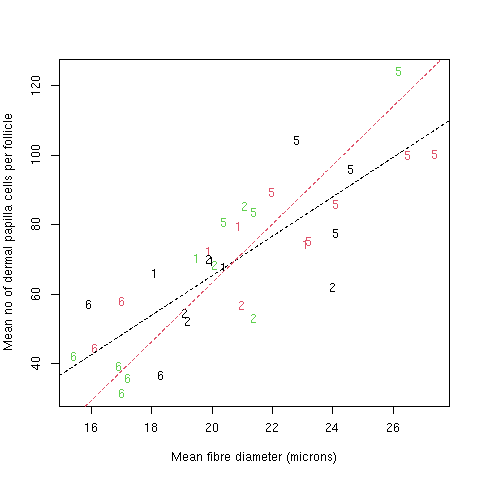
\includegraphics[width=0.9\textwidth]{dpccdiam2.png}
  \caption{Plot of mean fibre diameter against mean number of dermal papilla cells per follicle for 34 sheep from CSIRO selection experiments. The coloured numbers representing each point indicate the selection line (1 = high staple length, 2 = low staple length, 5 = high fibre diameter, 6 = low fibre diameter). The two dashed lines are   linear regressions of papilla cell count on diameter (black) and of diameter on papilla cell count (red).}
  \label{fig:dpccdiam}
\end{figure}

%\end{document}


 We can use this relationship to setup our starting values for average number of pre-papilla cells per follicle. Assume that the above relationship applies equally to all follicle types ( we have no information to the contrary), let us start with a sheep with $D_{P}=20$, $D_{So}=19$, and $D_{Sd}=18$ microns. The corresponding dermal papilla cell numbers are $C_{P}=65$, $C_{So}=59$, and $C_{Sd}=53$.  So we use these values as perhaps being typical of fine Merino sheep. We do not know if papilla cells continue to divide after they move to follicle bulbs and differentiate, so it is unclear whether the above data, which are for adult sheep, are relevant to estimating the number of pre-papilla cells actually used in forming a follicle in the foetus. For example, if there were one cell division after differentiation, the foetal numbers would be half the above estimates. We have no check on this.

There is other publishd data on dermal papilla cell numbers in follicles of other species. In mice, Chi, Wu, and Morgan(2013)~\cite{chi:13} observe that dermal papilla cell numbers vary between 20 and 100 per follicle, with guard hairs having more than other fibre types, and Zigzag fibres least. This agrees with our adult sheep estimates. The papilla cell numbers fluctuated with the mouse hair cycle, and their variation correlated with hair length and diameter. So the number of dermal papilla cells is not fixed for the life of a follicle, it can fluctuate with the hair cylcle, and fibre dimensionss fluctuate with it. Sheep are different from mice in that most of their follicles are in Anagen for long periods.  What we need to note here is a caution that adult dermal papilla cell numbers per follicle are not necessarily the numbers of pre-papilla cells used to initially form the follicle.

That leaves the parameter $C_{b}$, the probability that a cell chosen at random divides in unit time. We know nothing about this parameter for pre-papilla cells. We have chosen to make it a constant, but it may vary in unison with the changing growth rate of the whole foetus. We know that mammalian cells are capable of dividing about every 15 hours, but they do not all divide at that rate all the time. What we will do is complete the calculations outlined in Section~\ref{sec:calc} for a range of values of $C_{b}$, and with the other 19 parameters set as in Table~\ref{tab:base}, then see what value of $C_{b}$ gives a sensible result. We have chosen to specify this parameter as a probability, rather than as a mitotic rate, because that makes the calculation of number of new cells formed per unit time very simple, as is seen in equations~\ref{eqn:prim3}, ~\ref{eqn:so3}, and ~\ref{eqn:sd3}.

It turns out that results of our calculations a re remarkably sensitive to small variations in pre-papilla cell birth probability. Figure~\ref{fig:cbprobfn} shown the adult adult densities calculated from pre-papilla cell birth probabiltites ranging from 0.068 to 0.0769. 
%\documentclass{article}
%\usepackage{graphicx,subfigure}
%\begin{document}

\begin{figure}[!h]
  \centering
   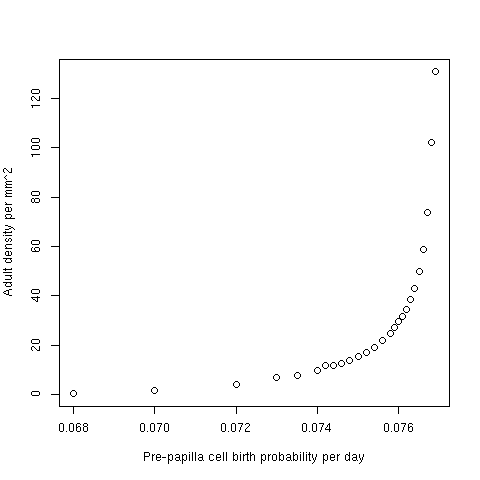
\includegraphics[width=0.9\textwidth]{cbprobfn.png}
%  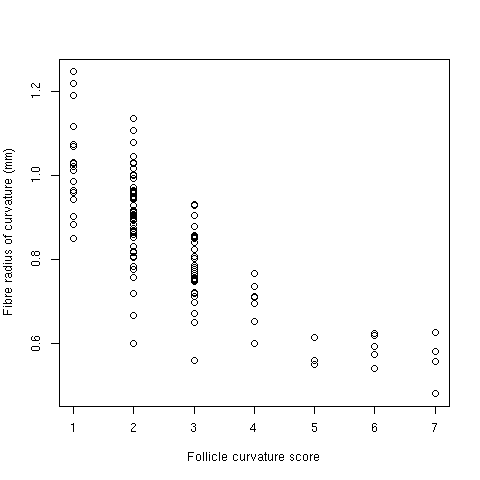
\includegraphics{ofdamm.png}
  \caption{Calculated values of adult follicle density from equations ~\ref{eqn:prim} to ~\ref{eqn:sd3} with values for parameters specified as for the first 19 parameters of Table~\ref{tab:base}, and with the $C_{b}$ parameter varying from 0.0680 to 0.0769}
  \label{fig:cbprobfn}
\end{figure}

%\end{document}


These adult densities cover the full range shown by all breeds of sheep from Wild sheep (5-10), to British breeds ( 15-25), to Australian Merinos ( 50-60), to SRS Merinos ( 60-70) follicles per square mm. To pick a base value for $C_{b}$ on this criterion we would go for about 0.0765, representing a modern Australian ( non-SRS) Merino. 

Figure~\ref{fig:cbprobsop} shows the same graph for adult S/P ratio. 
%\documentclass{article}
%\usepackage{graphicx,subfigure}
%\begin{document}

\begin{figure}[!h]
  \centering
   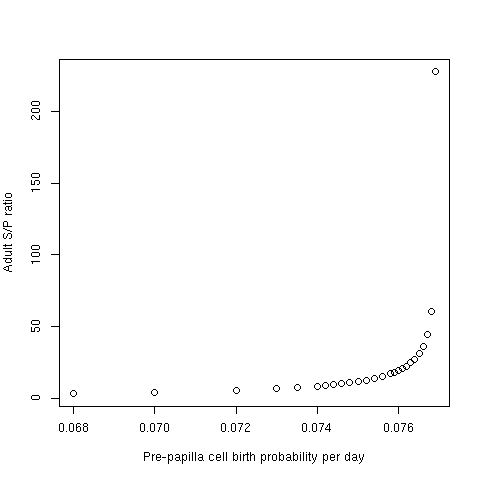
\includegraphics[width=0.9\textwidth]{cbprobsop.png}
%  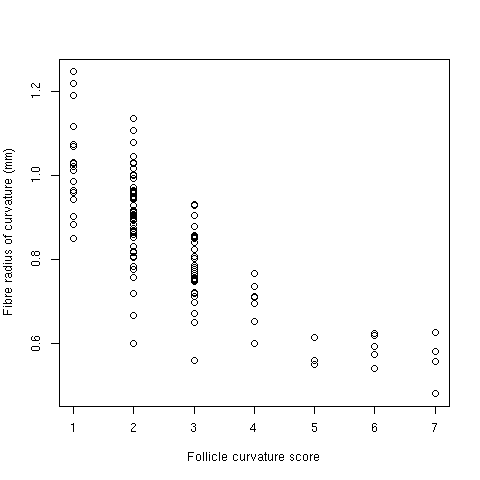
\includegraphics{ofdamm.png}
  \caption{Calculated values of adult S/P Ratio from equations ~\ref{eqn:prim} to ~\ref{eqn:sd3} with values for parameters specified as for the first 19 parameters of Table~\ref{tab:base}, and with the $C_{b}$ parameter varying from 0.0680 to 0.0769}
  \label{fig:cbprobsop}
\end{figure}

%\end{document}


The adult S/P ratios similarly cover the whole range fromWild sheep ( 3-5) , British breeds (5-6), Australian Merinos ( 15-30), and SRS Merinos ( 30-40). The S/P ratio rises rapidly to untenable values at high values of $C_{b}$, and if  $C_{b}$ is increased even further, what happens is that Sd follicles continue to form forever because the follicle intitation rate cannot keep up with the pre-papilla cell birth rate, and the pre-papilla cell pool is never exhausted. This , of course never happens in real sheep . To pick a base value for $C_{b}$ on the basis of S/P ratio we would go for about 0.0763, representing a modern Australian medium wool Merino. 

There is one further check on the feasability of our 20 starting parameters which we should look at briefly. That is the number of days over which follicle intitation proceeds for each of the P, So, and Sd follicle types. For P and So follicles, with our 20 starting parameters, the number of days of initiation is always 10, and 18 respectively. In other words primaries intitate from day 64 to day 73 and So's initiate from day 86 to day 103, both terminating when the number of sites runs out. However the days of initiation of Sd follicles varies with $C_{b}$. Sd initiation always starts when So initiation finishes ( day 105) but runs for 25 days with $C_{b}=0.0748$, 52 days with $C_{b}=0.0764$, and 69 days with $C_{b}=0.0767$. These and at days 130, 157, and 174 respectively. We know that most follicles are initiated by birth (150 days) so the day 174 may not be realistic, but no-one has ever studied follicle initiation in a high density Merino so we can not be sure.

The remarks made above relating calculated results for various $C_{b}$ values to breed means are not meant to imply that breed differences  in density and S/P ratio are caused by differences in $C_{b}$. Other parameters from Table~\ref{tab:base} could also produce such differences. We shall see this in the results below where we look at each parameter in turn. Here, we were simply trying to show that the calculated results were in the feasible region, if we chose certain values for $C_{b}$.

So we end with $C_{b}=0.0764$ as the base parameter value shown in Table~\ref{tab:base}, being half way between the values indicated from calculations of density and of S/P ratio. What does this mean? Well it says that on any one day 7.64 percent of the population of pre-papilla cells will divide. We have no idea if that is realistic, it simply makes the calculations work if we set it to that level. 

To put this tiny value $C_{b}=0.0764$ in perspective, it will produce a doubling of the cell population in about 10 days, because $(1.0765)^{10} = 2.08$.

We can now have a look at the detailed time series of development, as specified by the base parameter set. Figure~\ref{fig:basefollno} shows the cumulative numbers of each type of follicle initiated over the range of 60 to 900 days.
%\documentclass{article}
%\usepackage{graphicx,subfigure}
%\begin{document}

\begin{figure}[!h]
  \centering
   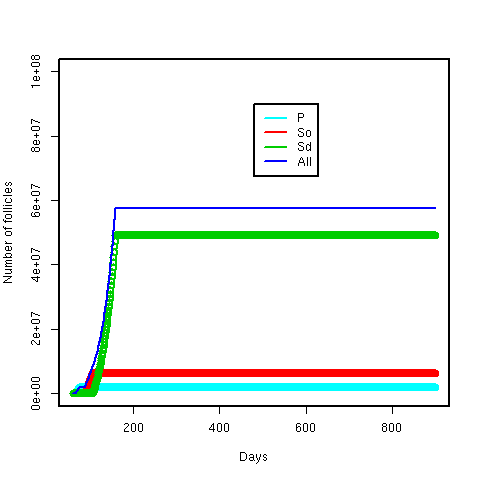
\includegraphics[width=0.9\textwidth]{basefollno.png}
%  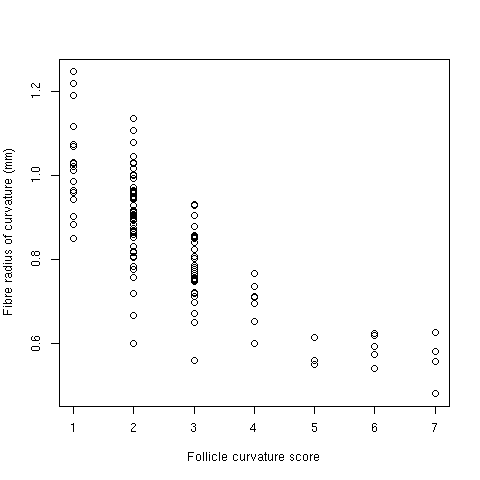
\includegraphics{ofdamm.png}
  \caption{Calculated values of follicle numbers at times from day 60 to day 900 from equations ~\ref{eqn:prim} to ~\ref{eqn:sd3} with values for parameters specified as for the 20 parameters of Table~\ref{tab:base}}
  \label{fig:basefollno}
\end{figure}

%\end{document}


We see the numbers rise to a maximum and then stay constant.
Figure~\ref{fig:basedens} shows the same time series for cumulative follicle densities. 
%\documentclass{article}
%\usepackage{graphicx,subfigure}
%\begin{document}

\begin{figure}[!h]
  \centering
   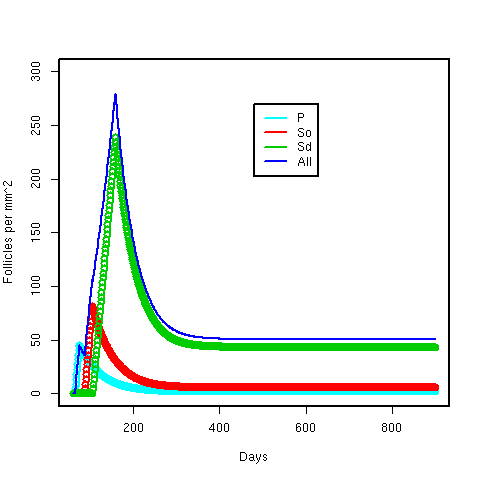
\includegraphics[width=0.9\textwidth]{basedens.png}
%  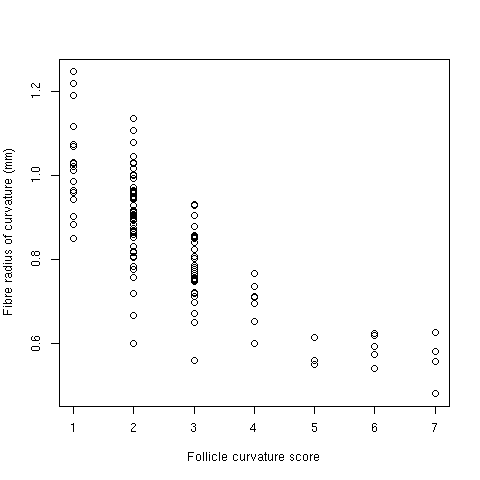
\includegraphics{ofdamm.png}
  \caption{Calculated values of follicle density at times from day 60 to day 900 from equations ~\ref{eqn:prim} to ~\ref{eqn:sd3} with values for parameters specified as for the 20 parameters of Table~\ref{tab:base}}
  \label{fig:basedens}
\end{figure}

%\end{document}


We see the densities rise to a peak, and then fall asymptotically as the sheep grows to adulthood.
Figures~\ref{fig:basefollno} and ~\ref{fig:basedens} are a reasonable description of how follicle development is known to proceed in the sheep.

We now accept our base parameter set, and move on to studying how varying each parameter affects the outcome.

\subsection{Effect of varying the initial number of pre-papilla cells}
Figure~\ref{fig:zcellnodens} show the adult density calculated at a range of values for parameter $(C_{n})_{0}$ which is the number of pre-papilla cells present at zero time. All other parameters are held constant at the base vales shown in Table~\ref{tab:base}.
%\documentclass{article}
%\usepackage{graphicx,subfigure}
%\begin{document}

\begin{figure}[!h]
  \centering
   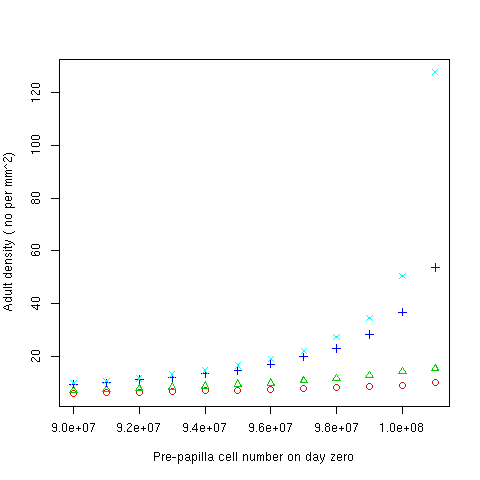
\includegraphics[width=0.9\textwidth]{zcellnodens.png}
  \caption{Calculated values of adult follicle density at a range of values of the parameter $(C_{n})_{0}$  from equations ~\ref{eqn:prim} to ~\ref{eqn:sd3} with values for the other 19  parameters fixed at the values given in Table~\ref{tab:base}. The four sets of points correspond to four values of the parameter $C_{b}$, red=.070, green=.073, blue=.076, cyan=.0764, the last being the base value for this cell birth probability parameter}
  \label{fig:zcellnodens}
\end{figure}

%\end{document}


We again see a calculated result which is sensitive to small variations in cell number at zero time. The effect of cell number at time zero is damped down if the cell birth probability is less than the base value of 0.074, and above 0.074 the process runs away and follicle initiation never ends. So the two parameters interact. Follicle formation is favoured by both a large starting number of pre-papilla cells, and by a high cell birth rate. Above $(C_{n})_{0}=1.1e+08$ the process runs away and follicle initiation never uses up all available pre-papilla cells. The Merino range is confined to 9.3e+07 to 1.0e+08.

Figure~\ref{fig:zcellnosop} shows a similar graph for adult S/P ratio. 
%\documentclass{article}
%\usepackage{graphicx,subfigure}
%\begin{document}

\begin{figure}[!h]
  \centering
   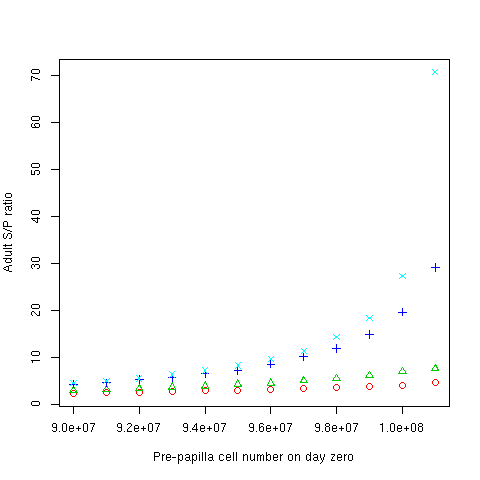
\includegraphics[width=0.9\textwidth]{zcellnosop.png}
  \caption{Calculated values of adult follicle S/P ratio at a range of values of the parameter $(C_{n})_{0}$  from equations ~\ref{eqn:prim} to ~\ref{eqn:sd3} with values for the other 19  parameters fixed at the values given in Table~\ref{tab:base}. The four sets of points correspond to four values of the parameter $C_{b}$, red=.070, green=.073, blue=.076, cyan=.0764, the last being the base value for this cell birth probability parameter}
  \label{fig:zcellnosop}
\end{figure}

%\end{document}


This is so close to the density graph that there is really nothing to add to what we said above.

It is clear that we can get to Merino levels of density and S/P ratio either by varing cell birth probability, or by haveing more pre-papilla cells available at time zero. This amounts to the same thing - if cell birth probability is high, the starting cell number is likely to also be high, because more cells will have divided before our time period.  We should probably reparameterize these two parameters into one, perhaps starting from one cell at an earlier time, and allowing the cell birth probability to control both. 

\subsection{Effect of varying the number of pre-papilla cells used to form a primary follicle}
Another way of promoting formation of more follicles, originally suggested by Philip Moore in 1979, and followed up assiduously by the SRS Merino breeding program, is to suppress the use of pre-papilla cells to form primary follicles, thereby making more pre-papilla cells available for cell division and for later formation of secondary follicles. This involves making primary follicles smaller, and is achievable by selection for low primary fibre diameter. 

The operation of ths effect is shown in Figure~\ref{fig:pavecellnodens}.
%\documentclass{article}
%\usepackage{graphicx,subfigure}
%\begin{document}

\begin{figure}[!h]
  \centering
   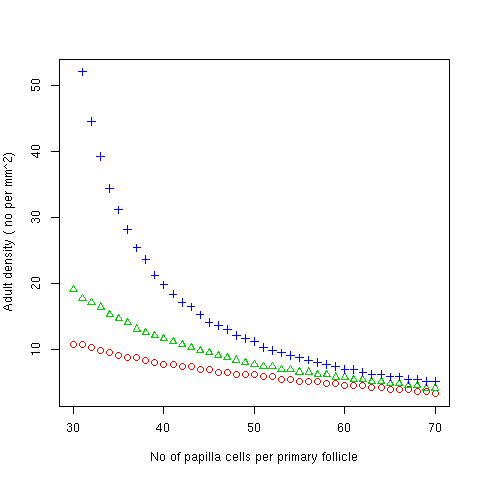
\includegraphics[width=0.9\textwidth]{pavecellnodens.png}
  \caption{Calculated values of adult follicle density at a range of values of the parameter $C_{P}$  from equations ~\ref{eqn:prim} to ~\ref{eqn:sd3} with values for the other 19  parameters fixed at the values given in Table~\ref{tab:base}. The three sets of points correspond to four values of the parameter $C_{b}$, red=.055, green=.060, blue=.064, the base value for this cell birth probability parameter being too high to use}
  \label{fig:pavecellnodens}
\end{figure}

%\end{document}


The effect is quite dramatic, and we have had to adjust the values of parameter $C_{b}$ downward to prevent the process from running away and making follicles forever. The base value of $C_{b}=0.074$ only works for values of no of papilla cells per primary follicle of 58 or greater, corresponding to primary fibres of diameter 18.7 or greater. The effect on  adult S/P ratio  is similar.

Modifying primary fibre diameter, in the fine direction, is a practical end effective way to achieve higher follicle densities. It is more effective if the diameter of secondary fibres is also kept fine.

\subsection{Effect of varying the number of pre-papilla cells used to form a secondary original follicle}
This is not practical, as So fibres or follicles cannot be reliably identified in adult skin biopsies. Nevertheless, we need to look and see what its effect would be, as it will be part of the effect of keeping all secondary fibres fine. Figure~\ref{fig:soavecellnodens} shows the effect on follicle density, with the values used for  $C_{b}$ being the same as in Figure~\ref{fig:pavecellnodens}
%\documentclass{article}
%\usepackage{graphicx,subfigure}
%\begin{document}

\begin{figure}[!h]
  \centering
   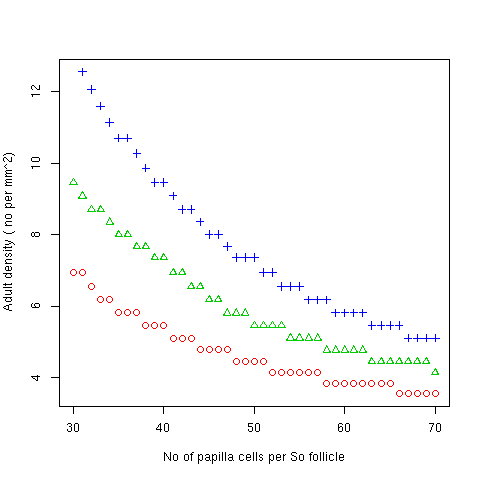
\includegraphics[width=0.9\textwidth]{soavecellnodens.png}
  \caption{Calculated values of adult follicle density at a range of values of the parameter $C_{So}$  from equations ~\ref{eqn:prim} to ~\ref{eqn:sd3} with values for the other 19  parameters fixed at the values given in Table~\ref{tab:base}. The three sets of points correspond to four values of the parameter $C_{b}$, red=.055, green=.060, blue=.064.}
  \label{fig:soavecellnodens}
\end{figure}

%\end{document}


We see that the effect of number of pre-papilla cells used by So follicles on adult follicle density is smaller than the effect  of a similar change in number of pre-papilla cells used by P follicles.  This is despite there being 3 times as many So follicles as P follicles. The effect is smaller because So follicles intitiate later than P follicles, so the opportunity for the unused pre-papilla cell population to multiply is reduced.  The effect on adult S/P ratio is similar.

\subsection{Effect of varying the number of pre-papilla cells used to form a secondary derived follicle}
This is more practical, as in Merino sheep most of the secondary fibres ( and therefore most of the fibres) are from Sd follicles. So one can simply reduce mean fibre diameter, or choose softer wool, and the effect will be to reduce the size of Sd fibres and follicles. Figure~\ref{fig:sdavecellnodens} shows the effect on adult follicle density, with the values used for  $C_{b}$ being the same as in Figure~\ref{fig:pavecellnodens}. 
%\documentclass{article}
%\usepackage{graphicx,subfigure}
%\begin{document}

\begin{figure}[!h]
  \centering
   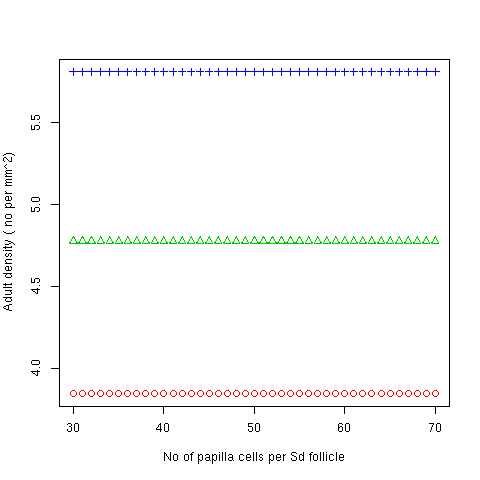
\includegraphics[width=0.9\textwidth]{sdavecellnodens.png}
  \caption{Calculated values of adult follicle density at a range of values of the parameter $C_{Sd}$  from equations ~\ref{eqn:prim} to ~\ref{eqn:sd3} with values for the other 19  parameters fixed at the values given in Table~\ref{tab:base}. The three sets of points correspond to four values of the parameter $C_{b}$, red=.055, green=.060, blue=.064.}
  \label{fig:sdavecellnodens}
\end{figure}

%\end{document}


 There is no effect at all, for these values of $C_{b}$.  Notice that the adult densities are small and in the non-Merino range. What is happening here is that the values for $C_{b}$ are too small, and there are no pre-papilla cells available to form Sd follicles, when So formation finishes. The three values of $C_{b}$ lead to different adult densities, because they vary how far the process proceeds through So initiation. Not all available So sites are being used here. The process is running out of cells during the So phase.

 If the pre-papilla cell birth probability is set to higher values, we see in Figure~\ref{fig:sdavecellnodens2} an effect of Sd papilla cell number on adult density. 
%\documentclass{article}
%\usepackage{graphicx,subfigure}
%\begin{document}

\begin{figure}[!h]
  \centering
   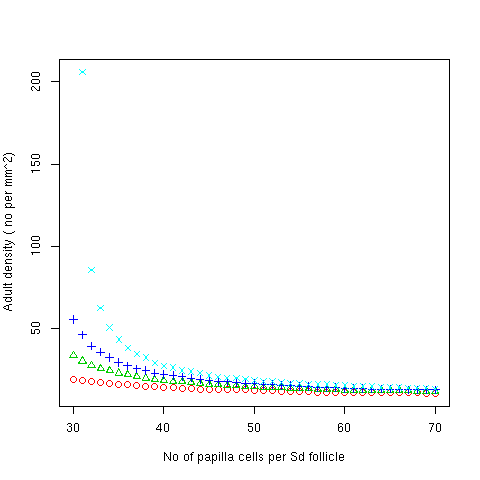
\includegraphics[width=0.9\textwidth]{sdavecellnodens2.png}
  \caption{Calculated values of adult follicle density at a range of values of the parameter $C_{Sd}$  from equations ~\ref{eqn:prim} to ~\ref{eqn:sd3} with values for the other 19  parameters fixed at the values given in Table~\ref{tab:base}. The three sets of points correspond to four values of the parameter $C_{b}$, red=.072, green=.073, blue=.0735, cyan=0.074}
  \label{fig:sdavecellnodens2}
\end{figure}

%\end{document}


Here we see that reducing the cells used by Sd follicles can increase adult density  , but the effect is only obvious when the number of pre-papilla cells per Sd follicle is reduced below about 40. 

The four levels of $C_{b}$ used in Figure~\ref{fig:sdavecellnodens2} cover the full range of effects. At $C_{b} > 0.074$ the process runs away and follicle initiation never ends. At values of $C_{b} < 0.072$ Sd follicles do not form at all, because the process runs out of pre-papilla cells in or at the end of the So initiation stage. That makes sense, but it is amazing how small a range of values for $C_{b}$ leads to realistic results in the Merino range. 

\subsection{Effect of varying number of pre-papilla cells used by all types of follicles}
If all the follicles use less pre-papilla cells ( equivalent to all the fibres being fine) we would expect an even larger effect on adult follicle density and S/P ratio. 

Figure~\ref{fig:avecellnodens} shows this effect for all three follicle types having the same papilla cell number and varying it over the range 30 to 70 cells per follicle.
%\documentclass{article}
%\usepackage{graphicx,subfigure}
%\begin{document}

\begin{figure}[!h]
  \centering
   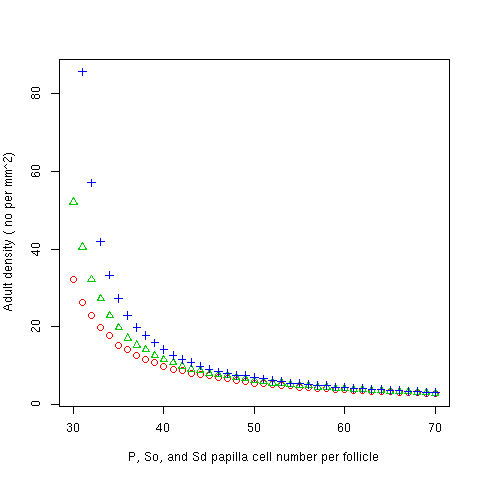
\includegraphics[width=0.9\textwidth]{avecellnodens.png}
  \caption{Calculated values of adult follicle density at a range of values of the parameters $C_{P}$ , $C_{So}$, and $C_{Sd}$,  from equations ~\ref{eqn:prim} to ~\ref{eqn:sd3} with values for the other 19  parameters fixed at the values given in Table~\ref{tab:base}. The three sets of points correspond to three values of the parameter $C_{b}$, red=.050, green=.052, blue=.054, the base value for this cell birth probability parameter being too high to use}
  \label{fig:avecellnodens}
\end{figure}

%\end{document}


We see quite a sharp effect at all three levels of the parameter $C_{b}$. We have had to change the levels of $C_{b}$ for this graph compared to Figures~\ref{fig:pavecellnodens}, ~\ref{fig:soavecellnodens}, and ~\ref{fig:sdavecellnodens2} to prevent the process running away and making follicles forever.

\subsection{Effect of varying follicle initiation rate}
The parameter $F_{r}$, has a base value of 450 follicles per $cm^{2}$ per time increment ( ie per day if $\delta t$ is set to 1). Note that this is on a per unit area basis. That means that the number of follicles formed per head per day increases as the foetus grows. 

Figure~\ref{fig:follinitratedens} shows the effect on adult density of varying parameter $F_{r}$ ( ie the follicle initiation rate) over the range 400 to 500, at 4 values of the parameters $C_{b}$.
%\documentclass{article}
%\usepackage{graphicx,subfigure}
%\begin{document}

\begin{figure}[!h]
  \centering
   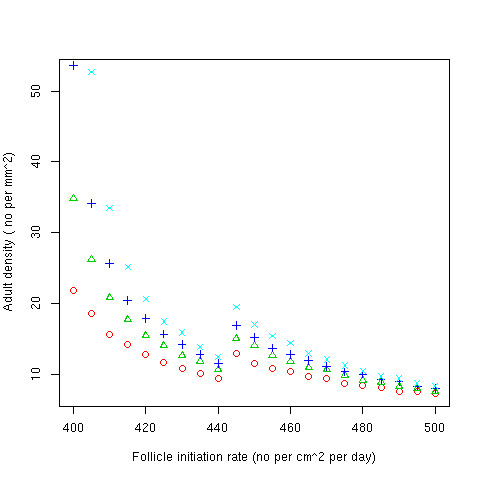
\includegraphics[width=0.9\textwidth]{follinitratedens.png}
  \caption{Calculated values of adult follicle density at a range of values of the parameter $F_{r}$  from equations ~\ref{eqn:prim} to ~\ref{eqn:sd3} with values for the other 19  parameters fixed at the values given in Table~\ref{tab:base}. The four sets of points correspond to four values of the parameter $C_{b}$, red=.072, green=.073, blue=.0735, cyan=0.074}
  \label{fig:follinitratedens}
\end{figure}

%\end{document}


Low follicle initiation rates lead to higher adult densities, because they slow down differentiation of pre-papilla cells and allow more cells to divide. 

Figure~\ref{fig:follinitratedens} has an unexplained step between $F_{r}=440$ and $F_{r}=445$.  Extensive investigation of behaviour of our equations and software around the region where the step occurs showed that there is no inconsistency. The equations do not have a singularity in the region where there is a step. It is simply a matter of the balance between cell use and cell formation - cell use is increased by the follicle initiation rate and by the numbers of cells used per follicle, while cell formation is increased by the cell birth probability.  There are two forces acting in opposite directions on follicle density, and in the middle of the follicle initiation rate range they interact nonlinearly.

That it is a question of balance can be illustrated by changing the foetal growth rate. If we modify parameter $B=.028$ which is the growth rate in our logistic growth equation, to a lower ( slower growth) value of $B=.024$, we get Figure~\ref{fig:slowfollinitratedens}
%\documentclass{article}
%\usepackage{graphicx,subfigure}
%\begin{document}

\begin{figure}[!h]
  \centering
   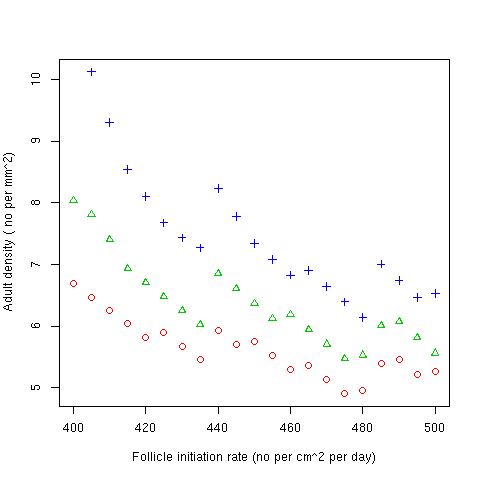
\includegraphics[width=0.9\textwidth]{slowfollinitratedens.png}
  \caption{Calculated values of adult follicle density at a range of values of the parameter $F_{r}$  from equations ~\ref{eqn:prim} to ~\ref{eqn:sd3} with values for the other 19  parameters fixed at the values given in Table~\ref{tab:base}. The three sets of points correspond to three values of the parameter $C_{b}$, red=.060, green=.062, blue=.064. The foetal growth rate in this graph has been changed from the base value of $B=.028$ to a slower value of $B=.024$.}
  \label{fig:slowfollinitratedens}
\end{figure}

%\end{document}


Here we see more than one step region. Changing the growth rate affects the effective follicle initiation rate because it is on a per unit area basis. The changed  effective rate interacts differently with the cell multiplication process.

\subsection{Effect of varying start times for follicle initiation}
Te parameters $T_{P}$ and $T_{So}$  are set to days 64 and 86 in the base parameter set. If we vary $T_{P}$ we need to vary $T_{So}$ in unison, so that the two waves of follicle initiation do not overlap.  We do this in Figure~\ref{fig:tptsodens}, settinf $T_{So} = T_{P} + 22 $. 
%\documentclass{article}
%\usepackage{graphicx,subfigure}
%\begin{document}

\begin{figure}[!h]
  \centering
   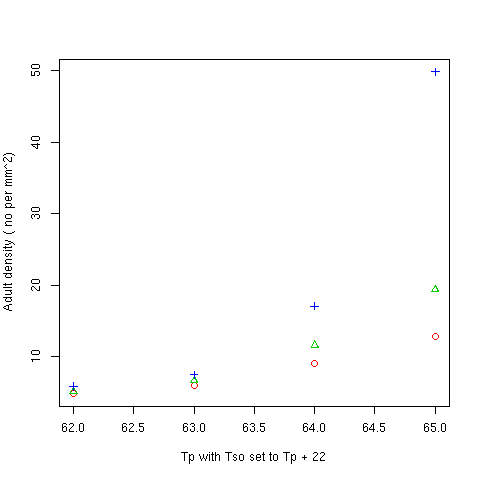
\includegraphics[width=0.9\textwidth]{tptsodens.png}
  \caption{Calculated values of adult follicle density at a range of values of the parameter $T_{P}$ ,  from equations ~\ref{eqn:prim} to ~\ref{eqn:sd3} with values for the other 19  parameters fixed at the values given in Table~\ref{tab:base}. The value of $T_{So}$ has been set to $T_{P}$ + 22 days. The three sets of points correspond to three values of the parameter $C_{b}$, red=.070, green=.072, blue=.074, the base value for this cell birth probability parameter being too high to use}
  \label{fig:tptsodens}
\end{figure}

%\end{document}


The effect is quite dramatic. Just shifting P and So initiation start times later by one day turns a Merino density of about 20 per $mm^{2}$ into a super Merino density of 50 per $mm^{2}$. Shifting earlier by one day turns a Merino into a non-Merino density of about 5 per $mm^{2}$. The timing of follicle development is critical

\subsection{Effect of number of sites}
We have almost arbitrarily set the parameter $L_{P}$ to $2$ x $10^{6}$ per head, and have said that there are 3 times as many So sites. In Figure~\ref{fig:lpdens} we look at varying $L_{P}$ . 
%\documentclass{article}
%\usepackage{graphicx,subfigure}
%\begin{document}

\begin{figure}[!h]
  \centering
   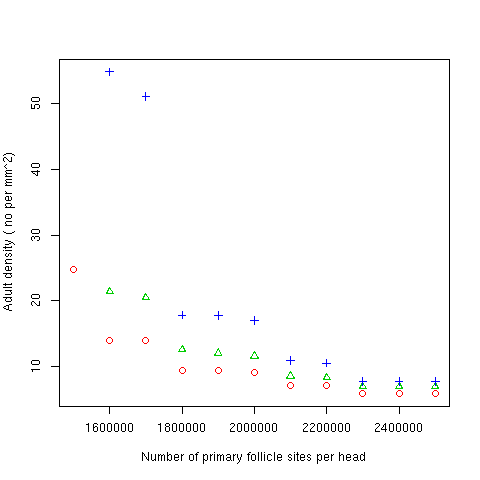
\includegraphics[width=0.9\textwidth]{lpdens.png}
  \caption{Calculated values of adult follicle density at a range of values of the parameter $L_{P}$ ,  from equations ~\ref{eqn:prim} to ~\ref{eqn:sd3} with values for the other 19  parameters fixed at the values given in Table~\ref{tab:base}. The three sets of points correspond to three values of the parameter $C_{b}$, red=.070, green=.072, blue=.074, the base value for this cell birth probability parameter being too high to use}
  \label{fig:lpdens}
\end{figure}

%\end{document}


Again we see a number of steps in the  plotted results. The overall result is clear, fewer primary sites has the same effect as using fewer pre-papilla cells to form a primary follicle, ie it leads to increase in the adult density.

It is not known if this effect operates in practice. Most sheep have number of primary follicles constant within a very narrow range, corresponding to adult primary densities of between 2.0 and 4.0 primaries per $mm^{2}$.

\subsection{Other parameters}
The remaining parameters have obvious effects. If we change the growth curve, particularly the growth rate, or the adult weight, then surface area is affected and there are consequences for follicle initiation rates and final densities. 

\clearpage
\section{Discussion}
The most obvious outcome of all of this numerical investigation is that the outcome we obtain is rather sensitive to changes in the 20 input paramters. The whole calculation is a delicate balancing act, and this is a reflection of a delicately balanced biological development process. 

Twenty parameters is quite a large number to describe a process that leads to just one or two numbers as an outcome. We would like to be able to turn the  calculation on its head and ask
\begin{quote}
"If a sheep has a certain density , S/P ratio, and fibre diameters ( Dp and Ds) what does that tell us about the range of values of the 20 starting parameters which could have led to this outcome?"
\end{quote}

We rather fear that the answer to the above question could be a wide range of values. There is no analytical method of doing the reverse calculation. The only thing we could do is choose a range of say 10 values of each parameter, run the calculation for all $20^{10}$ combinations, then search through all the results for those which match our nominated sheep.  $20^{10}$ is a daunting number of combinations (1.024e+13 to be exact).

We tried a more restricted set of parameter values. We left the growth parameters fixed , and held the numbers of papilla cells per follicle fixed ( effectively that holds fibre diameter fixed). We looked at 5 levels of each of the remaining 7 parameters. A mere $5^7 = 78125$ combinations. We then selected out those with a final density in a very narrow range ( eg 25 to 25.1) and found that just about all levels of each of the 7 parameters could lead to this result. We doubled the range of the 5 levels of each parameter and recomputed. Same result. What is happening is that if you choose one level of one parameter, the other 6 parameters just juggle around to force the resultant density to $25 to 25.1$. The parameters exhibit what is called redundancy - they are not all necessary as some can stand in for others and lead to the same effect.

It would be much more elegant for us to think a bit harder about the biology of development, and perhaps come up with a reparameterization to a smaller set of less redundant parameters. We have already noted that the number of pre-papila cells at time zero, and the cell birth probability must be related. Also the start times of development for P and So follicles must have a certain separation because P initiation always completes before So initiation starts. Quite a number of parameter combinations lead to results which 'run away', that is Sd initiation never ceases because the follicle initiation rate never catches up with the cell birth rate. That is clearly unbiological.  In the real world some of these partameters are clearly dependent on one another, and cannot be just chosen independently as we have rashly done in our calculations. Learning about that is the key to fixing it.



\clearpage
\begin{thebibliography}{99}

\bibitem{bogo:40}
 Bogolyubsky S.N. (1940) cited by Fraser A.S and Short B.F. (1960) The Biology of the Fleece. Animal Research Laboratories Technical Paper No 3. CSIRO Melbourne 1960.


\bibitem{cart:43}
Carter H.B. (1943) Studies in the biology of the skin and fleece of sheep. 1. The development and general histology of the follicle group in the skin of the Merino. 2. The use of tanned sheepskin in the study of follicle population density. 3. Notes on the arrangement, nomenclature, and variation of skin folds and wrinkles in the Merino. C.S.I.R. Bulletin No 164, Melbourne, 1943

\bibitem{cart:55}
Carter, H.B. (1955) The hair follicle group in sheep Animal Breeding Abstracts 23(2) 101-116

\bibitem{cart:68}
Carter,H.B. (1968) Comparative Fleece Analysis Data for Domestic Sheep. The Principal Fleece Staple Values of Some Recognised Breeds. Agricultural Research Council, 1968

\bibitem{chi:13}
Chi, W., Wu, E., and MOrgan, B.A. (2013) Dermal papilla cell number specifies hair size shae and cycling and its reduction causes follicular decline. Development 140(8):1676-1683

\bibitem{fras:60}
Fraser A.S and Short B.F. (1960) The Biology of the Fleece. Animal Research Laboratories Technical Paper No 3. CSIRO Melbourne 1960.

\bibitem{gord:08}
Gordon-Thompson, C., Botto, S.A., Cam, G.R., and Moore, G.P.H. (2008) Notch pathway gene expression and wool follicle cell fates. Aust. J. Exp. Agric. 48(5) 648-656

\bibitem{hard:56}
Hardy, M.H. and Lyne, A.G. (1956) The prenaltal development of wool follicles in Merino sheep. Aust. J. Biol. Sci. 9:423-441

\bibitem{jack:17}
Jackson, N. (2017) Genetics of primary and secondary fibre diameters and densities in Merino sheep. URL https://github.com/nevillejackson/atavistic-sheep/mev-rewrite/supplementary/genetic-parameters/psparam.pdf

\bibitem{jack:17a}
Jackson, N. (2017) Genetic relationship between skin and wool traits in Merino sheep. Part I Responses to selection and estimates of genetic parameters. URL https://github.com/nevillejackson/Fleece-genetics/tree/master/skinandfleeceparameters/ab3220/skinwool1.pdf


\bibitem{jack:90}
Jackson, N., Maddocks, I.G., Lax, J., Moore, G.P.M. and Watts, J.E. (1990) Merino Evolution, Skin Characteristics, and Fleece Quality. URL https://github.com/nevillejackson/atavistic-sheep/mev/evol.pdf 

\bibitem{jack:18}
Jackson, N. and Moore, G.P.H. (2018) R package {\em ppcell}. URL

\bibitem{madd:88}
Maddocks, I.G. and Jackson, N. (1988) Structural studies of sheep, cattle, and goat skin. CSIRO, Division of Aimal Production, Sydney.

\bibitem{metc:62}
Metcalf, J., Meschia, G., Hellegers, A., Prytowsky, H., Huchabee, W., and Barron, D.H. (1962) Observations on the growth rates and organ weights of fetal sheep at altitude and sea level. Quart. J. exp. Physiol. XLVII (4) 305-313

\bibitem{moor:89}
Moore G.P.M., Jackson, N., and Lax, J. (1989) Evidence of a unique developmental mechanism specifying both wool follicle density and fibre size in sheep selected for single skin and fleece characters. Genet. Res. Camb. 53:57-62

\bibitem{moor:98}
Moore, G.P.M., Jackson, N., Isaacs, K., and Brown, G (1998) J. Theoretical Biology 191:87-94

\bibitem{rprog:13}
R Core Team (2013). R: A language and environment for statistical
  computing. R Foundation for Statistical Computing, Vienna, Austria.
  ISBN 3-900051-07-0, URL http://www.R-project.org/.

\bibitem{ryde:68}
Ryder, M.L. and Stevenson, S.K.(1968) Wool Growth. Academic Press, London.

\bibitem{tapl:62}
Taplan, D.E., and Everitt, G.C. (1962) The influence of prenatal nutrition on postnatal performance of Merino lambs. Waite Agricultural Research Institute, University of Adelaide. 72-81 URL https://pdfs.semanticscholar.org/90b6/db6e9763d25add182220c0b369023072d41b.pdf

\bibitem{watt:18}
Watts, J.E., and Jackson, N. (2018) zIs collagen quantity and properties involved in wrinkle formation and/or in follicle development? URL https://github.com/nevillejackson/SRS-Merino/tree/master/supplementary/collagen/collagen.pdf

\bibitem{xavi:03}
Xavier, S.P., Gordon-Thomson, C. Wynn, P.C., McCullagh, P., Thomson, P.C., Tomkins, L., Mason, R.S., and Moore, G.P.M.(2003) Evidence that Notch and Delta expressions have a role in dermal condensate aggregation during wool follicle initiation. Experimental Dermatology, 22:656-681

\end{thebibliography}
\end{document}
